% Project report (IEEE two-column). Copied to report/latex/main.tex by `mmjee report`
% the first time only; edit report/latex/main.tex freely afterwards.
% Numbers come from generated_*.tex (regenerated on every `mmjee report`).
\documentclass[conference]{IEEEtran}
\usepackage{graphicx,booktabs,amsmath,url}
\usepackage[hidelinks]{hyperref}
\newcommand{\BaselineAcc}{43.2}
\newcommand{\SCAcc}{53.2}
\newcommand{\PoTAcc}{48.2}
\newcommand{\FullAcc}{65.3}
\newcommand{\BaselineNum}{40.2}
\newcommand{\PoTNum}{50.4}
\newcommand{\FullNum}{69.0}
\newcommand{\SCn}{20}


\begin{document}
\title{Improving Scientific Reasoning in Vision-Language Models using Code Sandboxes,
Agentic Correction, Learned Verification, and RAG on mmJEE-Eval}
\author{\IEEEauthorblockN{Arpit Kumar (12340350), Saurav Gupta (12341940)}
\IEEEauthorblockA{IIT Bhilai\\ \{arpitk, sauravg\}@iitbhilai.ac.in}}
\maketitle

\begin{abstract}
mmJEE-Eval is a bilingual multimodal benchmark of 1{,}460 JEE Advanced questions
(2019--2025). Its authors diagnose two weaknesses of vision-language models
(VLMs): unreliable numerical computation and a large gap between detecting and
fixing reasoning errors. We wrap a frozen open VLM in an inference-time framework
with four modules: a code sandbox (program-of-thoughts), an agentic
Solver/Critic/Corrector loop, a learned solution verifier for best-of-$N$
selection, and retrieval of worked exemplars. The verifier is the only trained
component; it is trained on automatically labelled solutions to the 2019--2024
questions. On the contamination-clean 2025 subset the single-pass baseline
reaches \BaselineAcc\% Pass@1, compute-matched self-consistency reaches
\SCAcc\%, and the full framework reaches \FullAcc\%.
\end{abstract}

\section{Introduction}
The base paper~\cite{mmjee} evaluates 17 VLMs and reports that open models
remain far behind frontier models on the held-out 2025 exam, and that models
fix only 1.1--5.2\% of the errors they detect in a single-pass
error-presence/error-correction protocol. It provides an evaluation harness but
no solver. We build a training-free (for the VLM) solver around a frozen model
and measure each module's additive effect, with a self-consistency
baseline~\cite{selfconsistency} at matched compute so that gains are not merely
due to more sampling.

\section{Data and Evaluation Protocol}
We use the public release (\texttt{ArkaMukherjee/mmJEE-Eval}). Questions are
images; metadata gives subject, type (MCQ-Single, MCQ-Multiple, Numerical,
Matching), year, paper and language. Training/development data are the
2019--2024 questions (1{,}270); all reported accuracies are on the 2025 subset
(190 = 95 English + 95 Hindi). Questions released after the paper (2026) are
not used. The base paper's answer-extraction (\texttt{extract\_answer}) and
scoring (\texttt{is\_answer\_correct}) functions are copied verbatim from its
notebooks; because the public data lacks the private columns these functions
read for range answers (e.g.\ ``8.70 TO 9.10''), we rebuild them on the data
side by expanding ranges on a 0.01 grid. Pass@1 is the mean accuracy over
independent samples (one ``run'' per sample index), as in the base paper.

\section{Method}
\subsection{Substrate}
The Solver is a frozen Qwen3-VL-8B-Instruct (AWQ 4-bit) served with vLLM on a
single 12\,GB GPU. The cross-model Critic is InternVL3.5-8B (AWQ 4-bit).

\subsection{Code-sandbox tool use}
Following program-of-thoughts prompting~\cite{pot}, the model reasons in numbered
steps and writes each calculation as a Python/SymPy program. Generation stops at
the end of every code block; the program is statically checked (import
whitelist, no file/process access) and executed in an isolated subprocess with
CPU, memory and wall-clock limits; its output is appended and generation
continues. If no \verb|\boxed{}| answer is produced, or code was attempted but
never ran, we fall back to the base paper's chain-of-thought prompt.

\subsection{Agentic iterative correction}
A Critic reads the image and the numbered steps and must name the \emph{first}
wrong step with a short explanation, instead of a yes/no verdict. The Corrector
(the Solver with the sandbox) keeps the accepted steps as a prefilled answer and
re-derives the solution from the located step, in the spirit of
Self-Refine~\cite{selfrefine}. The loop stops when the Critic finds no error,
when the answer is unchanged for two consecutive rounds, or after three rounds.
We compare a same-model and a cross-model Critic.

\subsection{Learned solution verifier}
We sample eight PoT solutions for every 2019--2024 question, label each with the
benchmark scorer against the gold answer, and train classifiers~\cite{cobbe}
that predict correctness from interpretable features (length, steps, code
success, CoT fallback, answer format and magnitude, agreement with sibling
samples) and a sentence embedding of the solution tail. We compare logistic
regression and XGBoost~\cite{xgboost} on three feature sets with GroupKFold
cross-validation on 2019--2023 (groups = question, so English and Hindi versions
never straddle folds) and select the configuration and selection rule
(max-probability or verifier-weighted vote) on the 2024 dev year. At test time
the verifier selects one answer from the pool of original and corrected
candidates.

\subsection{Retrieval-augmented exemplar prompting}
The Solver tags each question image with its topic and solution method. Tags of
2019--2024 questions index a knowledge base whose entries hold a transcription
of the problem and a Solver-generated worked solution verified by the scorer.
Entries that are near-duplicates of any 2025 question are removed. At inference
the top-2 same-subject entries above a similarity threshold (tuned on 2024
queries only) are added to the prompt as method guidance~\cite{rag}.

\section{Results}
\begin{table}[t]\centering\caption{Additive evaluation on the 2025 held-out subset (Pass@1, \%). $\Delta$: points vs.\ single-pass CoT.}\label{tab:main}
\begin{tabular}{lccc}\toprule
Configuration & Num. & Overall & $\Delta$ \\\midrule
Baseline (single-pass CoT) & 40.2 & 43.2 & -- \\
Self-consistency (matched compute) ($n{=}20$) & 51.2 & 53.2 & +10.0 \\
+ Code sandbox & 50.4 & 48.2 & +5.0 \\
+ Agentic correction (same-model critic) & 55.1 & 51.2 & +8.1 \\
+ Agentic correction (cross-model critic) & 53.0 & 51.3 & +8.2 \\
+ Learned verifier & 66.7 & 63.2 & +20.0 \\
+ Retrieval (RAG) & 69.0 & 65.3 & +22.1 \\
Full framework & 69.0 & 65.3 & +22.1 \\
\bottomrule\end{tabular}\end{table}

\begin{table}[t]\centering\caption{Verifier comparison (CV on 2019--2023, dev = 2024). Dev majority vote: 59.3\%.}\label{tab:verifier}
\begin{tabular}{llcccc}\toprule
Model & Feat. & CV AUC & Dev AUC & Dev F1 & Dev sel. \\\midrule
logreg & handcrafted & 0.893 & 0.916 & 0.844 & 61.3 \\
logreg & embedding & 0.672 & 0.706 & 0.698 & 59.3 \\
logreg & all & 0.891 & 0.915 & 0.847 & 61.8 \\
xgboost & handcrafted & 0.901 & 0.913 & 0.831 & 60.3 \\
xgboost & embedding & 0.677 & 0.689 & 0.687 & 57.8 \\
xgboost & all & 0.902 & 0.911 & 0.819 & 61.3 \\
\bottomrule\end{tabular}\end{table}


Table~\ref{tab:main} reports the additive evaluation. On Numerical questions the
code sandbox moves accuracy from \BaselineNum\% to \PoTNum\%; the full framework
reaches \FullNum\%. Self-consistency is evaluated with $n=\SCn$ CoT samples,
which matches the full framework's generated-token budget.
Table~\ref{tab:verifier} compares verifier models.

\begin{figure}[t]\centering
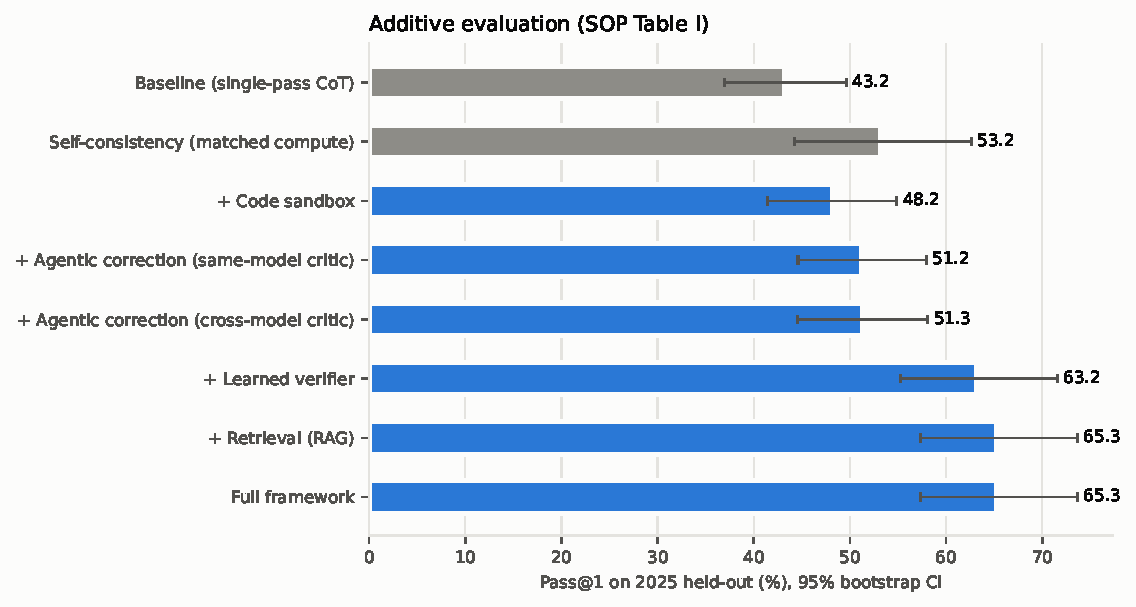
\includegraphics[width=\columnwidth]{../figures/table1.pdf}
\caption{Pass@1 with 95\% bootstrap confidence intervals.}
\end{figure}

\begin{figure}[t]\centering
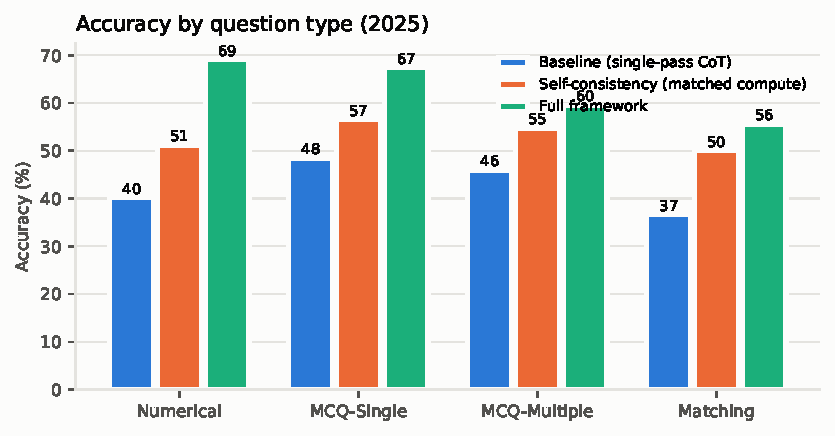
\includegraphics[width=\columnwidth]{../figures/per_type.pdf}
\caption{Accuracy by question type.}
\end{figure}

\begin{figure}[t]\centering
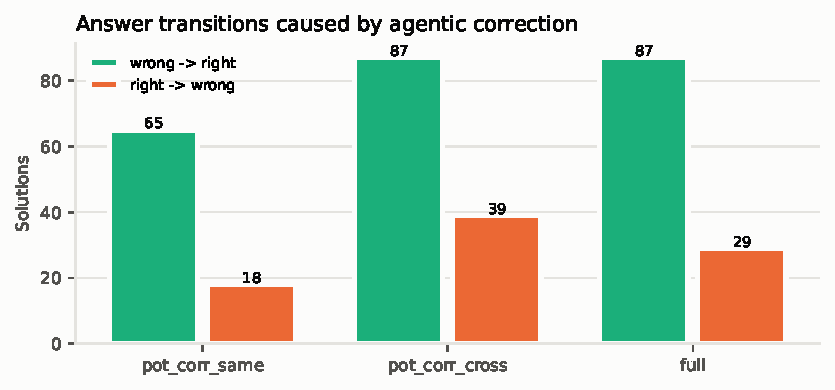
\includegraphics[width=\columnwidth]{../figures/correction.pdf}
\caption{Answer transitions produced by the correction loop.}
\end{figure}

\section{Discussion and Limitations}
% Write the discussion after inspecting REPORT.md. Points to cover: which module
% helps on which question type; correction fix vs. break rates compared with the
% base paper's 1.1--5.2%; verifier selection vs. majority vote at equal pool;
% retrieval coverage; compute cost; 190 questions give wide confidence intervals.
All conclusions are limited to one substrate model, one exam year (190
questions) and the base paper's strict scoring rules.

\section{Conclusion}
We implemented and evaluated a modular, verifier-guided, tool-augmented
multi-agent solver around a frozen VLM on mmJEE-Eval.

\appendix
\section{Prompts}
\paragraph{Baseline (base paper, English)}
\begin{small}\begin{verbatim}
Please analyze the image carefully, reason step-by-step and provide
your answer at the end.

For this question:
- Provide a numerical value
- Round to appropriate decimal places if needed
- Format your answer in \boxed{} (e.g., \boxed{2.5} or \boxed{42})
\end{verbatim}\end{small}

\paragraph{PoT solver instructions}
\begin{small}\begin{verbatim}
How to solve:
- Write the solution as numbered steps, each starting on a new line
with "Step 1:", "Step 2:", and so on.
- Explain the physics/chemistry/mathematics of each step in words.
- Do NOT do calculations in your head. Whenever a step needs a
calculation (arithmetic, algebra, solving equations, derivatives,
integrals, limits, unit conversions, or checking each option), write a
short Python program in a ```python code block that prints the result.
You may use math, fractions, sympy and numpy.
- End the code block with ```. The code will be run and its printed
output will be given back to you in an ```output block. Then continue
the solution using that output. Never invent the output yourself.
- Use at most 3 code blocks.
- Be concise: do not re-check the same step again and again.
- Finish with exactly one final answer in \boxed{}. Do not use \boxed
anywhere else. For a numerical answer write a plain decimal number
inside the box (no units, no fractions, no LaTeX), rounded to two
decimal places if it is not an integer.

Required format (example):
Step 1: <which law / concept applies and the equation to use>
```python
import sympy as sp
x = sp.symbols('x')
print(sp.solve(2*x - 6, x))
```
```output
[3]
```
Step 2: <interpret the printed result, check the options>
\boxed{<answer>}
\end{verbatim}\end{small}

\paragraph{Critic}
\begin{small}\begin{verbatim}
You are a strict examiner checking a student's solution to a JEE
Advanced question. The question is in the attached image{lang_note}.

Instructions the student was given:
{type_instruction}

Student's solution (steps are numbered):
<solution>
{solution}
</solution>

Check the steps in order: reading of the question and figure, chosen
concept and equations, algebra and arithmetic (the ```output blocks
are real program outputs), and the final option or number. Find the
FIRST step that contains an error. Do not solve the whole problem
again. Keep your check short (at most about 250 words), then end your
reply with exactly these three lines:
VERDICT: CORRECT or ERROR
FIRST_ERROR_STEP: <step number, or NONE>
EXPLANATION: <one or two sentences: what is wrong and how to fix it>
\end{verbatim}\end{small}

\paragraph{Corrector feedback}
\begin{small}\begin{verbatim}
A reviewer checked an earlier attempt at this question. The steps
before Step {k} were accepted and are already written at the start of
your answer. The reviewer found an error in Step {k}:
"{explanation}"
Continue the solution from Step {k}: re-derive that step correctly (do
not repeat the error) and complete the solution, following the same
rules (Python code for every calculation, one final \boxed{{}}
answer).
\end{verbatim}\end{small}

\paragraph{Concept tagger}
\begin{small}\begin{verbatim}
Look at this JEE Advanced exam question (it may be written in English
or Hindi). Do not solve it. In English, describe what is needed to
solve it, using exactly this format on one line:
SUBJECT: <Physics/Chemistry/Mathematics> | TOPIC: <specific topic, 2-6
words> | METHOD: <key concept or solution technique, at most 15 words>
\end{verbatim}\end{small}

\paragraph{Transcriber}
\begin{small}\begin{verbatim}
Transcribe this exam question exactly as plain text in its original
language. Write mathematical expressions in LaTeX. Include all answer
options. If there is a figure, add one line "[Figure: <short
description>]". Output only the transcription.
\end{verbatim}\end{small}

\paragraph{Exemplar header}
\begin{small}\begin{verbatim}
Below are worked solutions of earlier JEE Advanced problems that use a
similar method. Use them only as guidance on the method. They are
DIFFERENT problems: do not copy their numbers or answers.
\end{verbatim}\end{small}


\begin{thebibliography}{9}
\bibitem{mmjee} A.~Mukherjee and S.~Ghosh, ``mmJEE-Eval: A bilingual multimodal
benchmark for evaluating scientific reasoning in vision-language models,'' in
\emph{Findings of IJCNLP-AACL}, 2025.
\bibitem{pot} W.~Chen \emph{et al.}, ``Program of thoughts prompting,''
\emph{TMLR}, 2023.
\bibitem{selfrefine} A.~Madaan \emph{et al.}, ``Self-Refine: Iterative refinement
with self-feedback,'' in \emph{NeurIPS}, 2023.
\bibitem{cobbe} K.~Cobbe \emph{et al.}, ``Training verifiers to solve math word
problems,'' arXiv:2110.14168, 2021.
\bibitem{selfconsistency} X.~Wang \emph{et al.}, ``Self-consistency improves chain
of thought reasoning in language models,'' in \emph{ICLR}, 2023.
\bibitem{xgboost} T.~Chen and C.~Guestrin, ``XGBoost: A scalable tree boosting
system,'' in \emph{KDD}, 2016.
\bibitem{rag} P.~Lewis \emph{et al.}, ``Retrieval-augmented generation for
knowledge-intensive NLP tasks,'' in \emph{NeurIPS}, 2020.
\end{thebibliography}
\end{document}
